\section{One Hidden Layer Neural Network}

\subsection{Formulation for a Single Example}

\textbf{Forward Propagation:}

$z^{[1] (i)} =  W^{[1]} x^{(i)} + b^{[1]}$

$a^{[1] (i)} = g^{[1]}(z^{[1] (i)})$

$z^{[2] (i)} = W^{[2]} a^{[1] (i)} + b^{[2]}$

$\hat{y}^{(i)} = a^{[2] (i)} = g^{[2]}(z^{ [2] (i)})$

$y^{(i)}_{prediction} = \begin{cases} 1 & \mbox{if } a^{[2](i)} > 0.5 \\ 0 & \mbox{otherwise } \end{cases}$

\textbf{Cost}

$J = - \frac{1}{m} \sum_{i = 0}^{m} ( y^{(i)}\log(a^{[2] (i)}) + (1-y^{(i)})\log(1- a^{[2] (i)}))$

\textbf{Backward Propagation:}

$dz^{[2]} = a^{[2]} - y$

$dW^{[2]} = dz^{[2]} a^{[1]}$

$db^{[2]} = dz^{[2]}$

$da^{[1]} = W^{[2]^T} dz^{[2]}$

$dz^{[1]} = dz^{[1]} * g'^{[1]} (z^{[1]})$

$dW^{[1]} = dz^{[1]} x^T$

$db^{[1]} = dz^{[1]}$

\subsection{Vectorized Formulation}

\textbf{Forward Propagation:}

$Z^{[1]} =  W^{[1]} X + b^{[1]}$

$A^{[1]} = g^{[1]}(Z^{[1]})$

$Z^{[2]} = W^{[2]} A^{[1]} + b^{[2]}$

$\hat{Y} = A^{[2]} = g^{[2]}(Z^{[2]})$

\textbf{Cost}

$J = - \frac{1}{m} \sum ( Y * \log(A^{[2]}) + (1-Y) * \log(1- A^{[2]}))$

\textbf{Backward Propagation:}

$dZ^{[2]} = A^{[2]} - Y$

$dW^{[2]} = \frac{1}{m} dZ^{[2]} A^{[1]^T}$

$db^{[2]} = \frac{1}{m} \sum dZ^{[2]}$

$dA^{[1]} = W^{[2]^T} dZ^{[2]}$

$dZ^{[1]} = dA^{[1]} * g'^{[1]} (Z^{[1]})$

$dW^{[1]} = \frac{1}{m} dZ^{[1]} X^T$

$db^{[1]} = \frac{1}{m}  \sum dZ^{[1]}$

\subsection{Need for Non-Linear Activations}

If we have linear activation functions, then our output is just a linear combination of the input features. Therefore, no matter how many layers we include, we would just get a standard linear regression.

\subsection{Activation Functions}

\vspace{0.25cm}

\begin{multicols}{2}
\begin{centering}

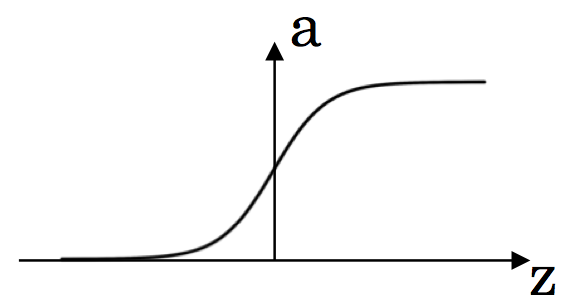
\includegraphics[width=2.5cm]{images/sigmoid.png}

sigmoid

$a = \frac{1}{1 + e^{-z}}$

$g'(z) = a(1-a)$

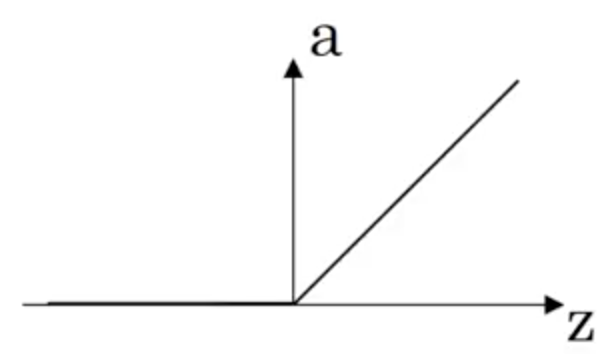
\includegraphics[width=2.5cm]{images/relu.png}

ReLU

$a =  \max (0, x)$

$g'(z) = \begin{cases} 0 & \mbox{if } z < 0 \\ 1 & z \geq 0 \end{cases}$

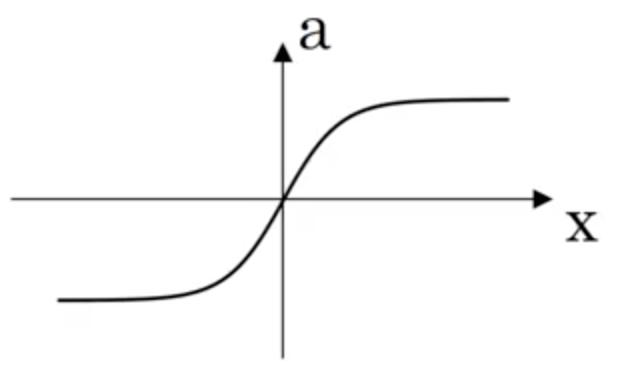
\includegraphics[width=2.5cm]{images/tanh.png}

tanh

$a = \frac{e^z - e^{-z}}{e^z + e^{-z}}$

$g'(z) = 1-a^2$

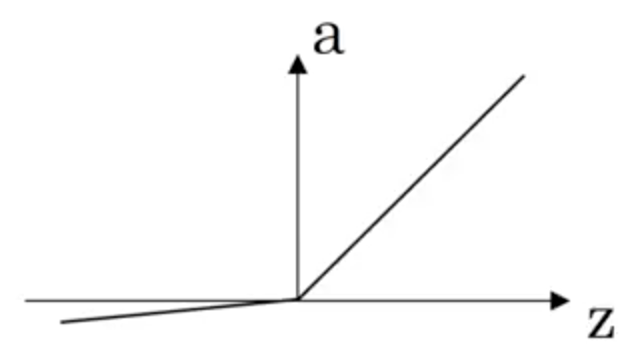
\includegraphics[width=2.5cm]{images/leaky_relu.png}

Leaky ReLU

$a =  \max (0.01x, x)$

$g'(z) = \begin{cases} 0.01 & \mbox{if } z < 0 \\ 1 & z \geq 0 \end{cases}$

\end{centering}
\end{multicols}

\vspace{0.1cm}

\subsection{Random Weight Initialization}

\begin{itemize}[wide, labelwidth=!, labelindent=0pt]
\itemsep0em 
    \item In logistic regression it wasn't important to initialize the weights randomly, while in a neural network with more than one layer we have to initialize them randomly.
    \item If we initialize all the weights with zeros, then on each gradient descent iteration all the hidden units will always update the same way. This means all hidden units will be completely identical and won't be able to break symmetry.
    \item We initialize weights with small random values in [0, 0.01].
    \item If weights are too large, then we end up on the edges of tanh or sigmoid activation function, so learning is slow. 
    \item We can initialize biases to 0 and still break symmetry. \vspace*{-\baselineskip}
\end{itemize}
